% !Mode:: "TeX:UTF-8"
%!TEX program  = xelatex

\documentclass[bwprint]{gmcmthesis}

\usepackage{threeparttable}
\usepackage{enumitem}
\usepackage{algorithmic}
\usepackage{algorithm}
\usepackage{float}


\usepackage[framemethod=TikZ]{mdframed}
\title{出版社图书印制策略}
\baominghao{xxxx} %参赛队号
\schoolname{中国地质大学(武汉)}%学校名称
\membera{李延炽} %队员A
\memberb{熊诗捷} %队员B
\memberc{明飞} %队员C
\begin{document}

 %生成标题
 \maketitle

 %填写摘要
\begin{abstract}
汽油在生产生活中有着难以取代的作用。

\keywords{数据挖掘\quad 遗传算法}
\end{abstract}

\pagestyle{plain}

%目录 不推荐加
%\tableofcontents

\section{问题重述}

\subsection{引言}

某出版社出版发行与初等教育相关的图书, 在运营过程中, 遇到了图书印量、图书销售量和图书库存之间如何协调的问题。在印制图书的时候,除了根据印量会产生纸张费、印刷费、装订费、封面工艺费等印刷成本外,每一次印刷都有一笔数千元的上版费,因此出版社自然希望一次开机尽量多印一些,但是图书销售量通常是不确定的,如果印多了,图书库存加大,会导致与库房结算的发货费率*(见注1中定义)提升,增大发货费用;滞销图书等待报废,其印刷成本的投入会全部损失殆尽。因此,一本书印几次,每次印多少,是这个出版社希望解决的问题。为此,请你们为该出版社出谋划策,仅考虑印刷成本和库房发货费用。针对不同类型的图书提供最优的印刷方案,以期获得尽可能大的销售收益。

\subsection{问题的提出}

该出版社出版发行的图书主要分A、B、C三类。

A类图书属于政府采购类(如经国家审批出版的教材教辅),不面向市场公开销售。这类图书定价低(销售折扣约48\% 折),订单数量大且相对稳定,但图书更新快,当年的滞销书成为库存,等待报废。现有问题是:订单上报时间不集中,且收到订单后通常需要迅速发货,在征订后期经常有几百册的增补订单,导致印次能多达7-8次。

B类图书是直销类图书,主要用于高考复习使用,直接进校推广。这类图书定价高,销售折扣低(销售折扣约18\% 折),图书更新快,当年不能销售的书成为滞销库存,等待报废。现有问题是:这类图书因定价高,滞销库存总体码洋*(见注1中定义)较大,对发货费率影响较大。

C类是市场零售类图书,走实体书店和网上渠道销售,没有特别集中的订量,销售不可控。这类图书销售折扣约45\% 折,定位于长销,销售时间可延续若干年,但通常图书上市2年以后,热度就会减弱,如果处于滞销状态,就会等待报废。现有问题是:该类图书的首印通常在3000-5000册,如果能够实现全部销售,则一定处于盈利状态,当某本图书库存不足500册时,会考虑重印,出版社希望能根据上一次印刷后的销售情况,并结合热度衰减因素,来规划下一次的印刷数量,使其实现盈利增加。

出版社与库房结算的发货费率每年调整一次,取值范围如注1名词解释中表格所示。可以假设发货费率在近几年保持不变,而当前的发货费率为2.73\%。

请建立数学模型,完成下面的任务:

1. 研究A类图书的需求和订单规律(附件1),对每本书给出2021年秋或者2022年春的最优印刷方案。有没有可能将总印次控制在3次以内? 

2. 对B类图书,根据往年的销售情况(附件2),在降低库存的前提下,对每本书给出下一年度的最优印刷方案。

3. 对C类图书,对附件3中的9本图书,考虑未来可能的销售情况,给出每本书的重印方案(是否需要重印,如需重印,最优重印数量),并判断出版社之前的重印策略是不是最优的。

4. 给该出版社写一个企划书,对图书的印刷方案给出你们的建议。

题中包含若干名词解释和行业约定

【注 1】 名词解释

码洋:图书的定价×数量

滞销库存码洋:图书的定价×滞销库存数量

上版费:指印刷开机前,需要将图书文件上机制版产生的费用,上版费与图书的印张有关,可利用附件4的《图书印制成本计算表》计算。

销售率:(发货数量-退货数量)/印刷数量

发货费率:用于和库房结算库租物流费用(又称库房发货费用)的一项指标, 与出版社所有图书全年发货码洋和每个月的平均库存有关,也即和图书的周转情况有关。图书周转越快,库存图书码洋越少, 发货费率越低;反之,图书周转越慢,库存图书码洋越多, 发货费率越高。每年的发货费率对所有图书都是一个固定的常数,部分取值如下表所示:

\begin{table}[htbp]
\resizebox{\textwidth}{!}
{
\begin{tabular}{|cccccccccc|}
\hline
100\%-91\% & 90\%-81\% & 80\%-71\% & 70\%-61\% & 60\%-51\% & 50\%-41\% & 40\%-31\% &30\%-21\%  & 20\%-11\% & 10\%-0\% \\
\hline
3.42\% & 3.12\% & 2.91\% & 2.73\% &	2.60\% & 2.48\% & 2.40\% & 2.32\% & 2.25\% & 2.19\% \\
\hline
\end{tabular}
}
\caption{发货费率取值表}
\label{tab:sr}
\end{table}

目前该出版社所有图书的发货费率结算标准是2.73\%。

库房发货费用:即库租物流费用,计算公式是:

发货费用=发货数量×定价×发货费率

(注:发货数量+滞销库存数量=印刷数量)

利润=定价×印数×销售折扣×销售率-(印制成本+库房发货费)			


【注 2】 行业约定

    当印刷数量低于2000册时,因印刷开机成本问题,印刷企业会按照2000册印量进行计费。所以,低于1500册时,通常会采用数码印刷,数码印刷费用会较传统印刷费用上浮15\%。

\newpage

\section{符号说明}
\begin{tabular}{ccc}
	\hline
	\makebox[0.1\textwidth][c]{符号}	&  \makebox[0.35\textwidth][c]{意义} &\makebox[0.35\textwidth][c]{注释} \\ \hline
	$A1\textasciitilde A5$	    & A类图书5本 & $1-5$表示图书编号 \\ \hline
	$B1-1\textasciitilde B1-5$	    & B类图书第一类5本 & $1-5$表示图书编号 \\ \hline
	$B2-1\textasciitilde B2-5$	    & B类图书第二类5本 & $1-5$表示图书编号 \\ \hline
	$C-1\textasciitilde C-9$	    & C类图书9本 & $1-9$表示图书编号 \\ \hline
	$pc$	    & 图书定价 & 参照附录1-3确定定价  \\ \hline
	$N$	    & 印刷数目/印数 &   \\ \hline
	$d$	    & 折扣率 & d\% \\ \hline
	$s$	    & 销售率 & s\%  \\ \hline
	$c$	    & 印制成本 &   \\ \hline
	$sc$	    & 库房发货费 &   \\ \hline
	$pf$	    & 利润 &  \\ \hline
	$sv$	    & 图书销量 &   \\ \hline
	$sq$	    & 发货数量 &   \\ \hline
	$uns$	    & 滞销库存数量 &   \\ \hline
	$rq$	    & 退货数量 &   \\ \hline
	$sr$	    & 发货费率 & sr\% \\ \hline
	$srp$	    & 发货占比 & srp\%  \\ \hline
	$S$	    & 当前库存 &  \\ \hline
	$ra$	    & A类图书订单需求 &  \\ \hline
	$s_s$	    & 安全库存值 &   \\ \hline
	$p^k_f$	    & A类图书Ak首单占比 & 首单为首大订单及其增补  \\ \hline
	$er$	    & 预测值与实际值的误差率 & er\%  \\ \hline
\end{tabular}
\newpage

\section{问题分析与模型假设}

依据题目意思,最终的目标函数是求得出版社在给定方案下的运营利润。

假设定价为$pc$,印刷数量为$N$,销售折扣率$d\%$,销售率$s\%$,印制成本$c$,库房发货费$sc$。利润$pf$的计算方式如下:
\begin{equation}
\label{eq:pf}
  pf = pc\times N\times d\times s - (c + sc),
\end{equation}	

其中,定价$pc$可参照附录1-3找得;印刷数量$N$计算如下:
\begin{equation}
\label{eq:N}
  N = sq + uns,
\end{equation}
其中,$sq$代表发货数量、$uns$代表滞销库存数量;销售折扣率$d\%$参照题目文本;以$sv$代表销量,则销售率$s\%$计算方式如下:
\begin{equation}
\label{eq:s}
  s = sv / N = (sq - rq) / N,
\end{equation}
其中,$rq$代表退货数量;印制成本$c$可通过附录4的excel表格计算,主要关联因素为印张、装订方式及印刷方式;库房发货费$sc$计算方式如下:
\begin{equation}
\label{eq:sc}
  sc = sq\times pc\times sr,
\end{equation}
其中,$sr$表示发货费率,在本文中,因为发货费率是由图书周转情况确定,为简化计算,发货费率通过发货数量占比划分区间确定,占比$srp$的计算方式为:
\begin{equation}
\label{eq:srp}
  srp = sq / N,
\end{equation}
根据此占比值,发货费率由表格~\ref{tab:sr}~确定。依据题意假设,目前该出版社所有图书的发货费率结算标准是2.73\%。


\subsection{问题一}

A类图书属于政府采购类(如经国家审批出版的教材教辅),不面向市场公开销售。这类图书定价低(销售折扣约48\% 折),订单数量大且相对稳定,但图书更新快,当年的滞销书成为库存,等待报废。现有问题是:订单上报时间不集中,且收到订单后通常需要迅速发货,在征订后期经常有几百册的增补订单,导致印次能多达7-8次。

问题一的题目要求:

研究A类图书的需求和订单规律(附件1),对每本书给出2021年秋或者2022年春的最优印刷方案。有没有可能将总印次控制在3次以内? 

\subsubsection{问题分析}

问题一所求为A类图书中,A1-A5五本图书下一年的季度性印刷方案。要求在保证发印刷数量大于当前订单需求,即$N>mr$的情况下,给出每一本书在下一年的最优印刷方案。A类图书的运营效果由最终方案带来的利润评估。

A类图书是不面向市场销售的政府采购类,其特点是订单零散,但需要接单后尽快发货。A类图书印刷的主要矛盾存在于不确定的订单造成的高印次带来的上版费等开销,导致最终成本增加。问题一的主要目的是针对A类图书的每本书给出印刷方案,力求将总印次控制在3次以内,同时达到利润最大化。

通过对附录1的数据观察,我们总结出问题一的如下特征:
\begin{itemize}
  \item 印刷产生在某一年的一个季度之内(春季1-3月份,秋季7-9月份),总体而言是对季度前及季度中的订单的生产;
  \item 由于订单分散、且时间不确定,某些图书为了满足订单需求往往在一个季度内印次在1-6次不等,且末尾几次印刷数量小($N<2000$);
  \item 除开数量相对来说极少的增补订单外,A类图书的印刷数量绝大部分是为了满足前期的大订单;
  \item A1-A5不同图书的订单虽然零散,但总数相对稳定,且往年数据或相对平稳,或存在一定的逐年变化趋势;
  \item 由于A类图书定价低,但接到订单后能迅速发货,因此其发货费率较低,但印次带来的上版费高,所以影响A类图书利润的主要因素是不确定的订单需求造成的高印次。
\end{itemize}

因此,对问题一的求解,我们希望能够结合现有数据,有效分析下一年一个季度里每个月的订单总数,根据预测的订单数执行印刷计划,旨在短期储备库存,避免需求少而订单多造成的多印次。大体的做法如下:
\begin{itemize}
  \item \emph{Step 1:}根据往年数据中的订单报数年度总和,预测下一年的订单总数,作为印刷总数;
  \item \emph{Step 2:}在安全库存的模型基础上,通过分析本题中问题的特性和数据的特点,确定存储供应周期和额外安全库存量的预测方式;
  \item \emph{Step 3:}根据第二步得到的安全库存模型,制定印刷策略,产生具体印刷方案;
  \item \emph{Step 4:}以往年的数据,产生该模型下的新印刷方案,通过计算利润验证模型精度,进行修正;
  \item \emph{Step 5:}基于往年数据预测下一年的订单分布,并根据提出的安全库存模型预估利润。
\end{itemize}

\subsubsection{模型假设}

根据题意信息,在求解问题一时,我们保持如下的基本假设:

\begin{itemize}
	\item 发货费率在近几年保持不变,当前的发货费率为2.73\%;
	\item A1-A5五本图书的印刷量、销量等之间均无相关关系;
	\item 基于存储周期根据预测值印刷的方法,销售量以附录1中的订单报数为准,所有时间相近或印刷数量较少的订单视作时间上最接近的大订单的增补;
	\item 不考虑A类图书的订单印刷时间,即订单上报后能短期内完成印刷并发货;
	\item 不考虑存储供应周期内印刷时间到订单时间差造成的延误带来的经济损失;
	\item 发货费率的计算以表~\ref{tab:sr}~为准。
\end{itemize}

\subsection{问题二}

B类图书是直销类图书,主要用于高考复习使用,直接进校推广。这类图书定价高,销售折扣低(销售折扣约18\% 折),图书更新快,当年不能销售的书成为滞销库存,等待报废。现有问题是:这类图书因定价高,滞销库存总体码洋*(见注1中定义)较大,对发货费率影响较大。

问题二的题目要求是:

对B类图书,根据往年的销售情况(附件2),在降低库存的前提下,对每本书给出下一年度的最优印刷方案。

\subsubsection{问题分析}

问题二所求为B类图书中,B1类和B2类各五本的印刷方案。要求在降低库存的前提下,给出每本书下一年度的最优印刷方案。而同样的,问题二中B类图书的运营效果由最终方案带来的利润评估。

B类图书是定价高且销售折扣低的类型,高定价容易造成库存总体码洋大,进而增大发货费率最终导致发货成本高。题目要求主要目的为在降低库存的前提下,求得满足销售需求的印刷方案。也就是尽量让印刷发货出去的成品满足该时段销售量需求从而减少库存,降低成本。由此可见该题中主要矛盾在于:高定价使库存要求严格,即产即销是最优的方案。

通过观察附录2的数据,我们总结出问题二的如下特征;

\begin{itemize}
  \item B1类图书的销售周期是3月到9月,其实际销售情况与之相符;同样的,B2类图书的销售周期是10月到次年4月,其实际情况与之大致相符;
  \item B1类图书在每周期的4-8月,B2类图书在每周期的12-1月往往供不应求(印刷多,卖的也多),导致中途加印,而其他月份供大于求,库存积压;
  \item 在销售周期的结束月,销量往往开始剧减,周期结束后直到下一周期开始,销量较之之前同样剧减;
  \item 图书的印次大体上一年更新两轮(比如1-1到1-3),修订的结果往往是印张的调整,从而导致印刷成本变化;
  \item 印次为偶数的版本,依照题目意思可以不做讨论,故归入其他印次版本;
  \item 销量统计以月为单位,可见销售周期内均可满足$sv$≥2000的条件;而销售周期外均不能满足该条件;
  \item 不考虑2020年1月开始的新冠疫情影响,数据整体走势明显,且显示出较为稳定的变化趋势。
\end{itemize}

因此对于问题二的求解,我们希望能够结合现有数据,有效分析下一年图书的销量,主要为销售周期内,每个月的销量,而同时将非销售周期内的图书销量并入周期末尾月。以此为基础制定印刷计划。旨在减少库存量,实现图书尽可能的即印即销。大体做法如下:

\begin{itemize}
  \item \emph{Step 1:}对往年数据做加工处理,将原本的每年销量转换为按照销售周期,每个周期销量;
  \item \emph{Step 2:}在销售周期内按照月份统计每月销售量,将非周期的销量并入周期末月(9月和4月),然后构建销量趋势预测;
  \item \emph{Step 3:}以前两步的数据为基础预测下一年销售周期内的年销量,以此决定印刷数量;
  \item \emph{Step 4:}基于经济订购批量模型(EOQ),为下一年的印刷制定最优的印刷方案;
  \item \emph{Step 5:}根据往年印次变化,确定当年印次参数,并计算印刷成本,
  \item \emph{Step 6:}以往年的数据验证模型精度,进行修正;
  \item \emph{Step 7:}预估方案下,计算下一年的运营利润;
\end{itemize}

\subsubsection{模型假设}

根据题意信息,在求解问题二时,我们保持如下的基本假设:

\begin{itemize}
	\item 发货费率在近几年保持不变,当前的发货费率为2.73\%;
	\item B1,B2两类各五本图书之间无相关关系;
	\item 由于往年积压图书报废,可忽略库存,直接从附录2取得每月销量;
	\item 印次的变化符合往年变化总趋势,不会出现特殊情况;
	\item 印次为偶数的配套的教师用书,可并入前一印次,根据题意不做讨论;
	\item 不考虑月内发货和印刷时间差造成的延误带来的经济损失;
	\item 各种购物途径下,可以忽略新冠疫情等外界因素带来的影响。
\end{itemize}

\subsection{问题三}

C类是市场零售类图书,走实体书店和网上渠道销售,没有特别集中的订量,销售不可控。这类图书销售折扣约45\% 折,定位于长销,销售时间可延续若干年,但通常图书上市2年以后,热度就会减弱,如果处于滞销状态,就会等待报废。现有问题是:该类图书的首印通常在3000-5000册,如果能够实现全部销售,则一定处于盈利状态,当某本图书库存不足500册时,会考虑重印,出版社希望能根据上一次印刷后的销售情况,并结合热度衰减因素,来规划下一次的印刷数量,使其实现盈利增加。

问题三的题目要求是:

对C类图书,对附件3中的9本图书,考虑未来可能的销售情况,给出每本书的重印方案(是否需要重印,如需重印,最优重印数量),并判断出版社之前的重印策略是不是最优的。

\subsubsection{问题分析}

问题三所求为C类图书中,C1-C9九本图书图书的重印方案,并评估往年的重印策略是否最优。要求根据上一次印刷后的销售情况,结合热度衰减因素,规划下一次的印刷数量,使其实现盈利增加。同样,问题三中C类图书的运营效果由最终方案带来的利润评估。

C类图书是市场零售类图书,销量不可控制,即没有稳定数值。由于图书定位于长期销售,在销售过程中会出现重印发货的需求。当库存$uns<500$时,出版社就需要考虑重印以准备满足后续的销售需求。此时需要对下一次是否重印、重印数量进行预测分析。本题关键在于,销售量没有稳定数值或趋势,但销售过程中,存在热度衰减的规律。因此,问题三的目标为,规划每本图书是否重印及重印数量,使利润最大化。

通过观察附录3的数据,我们可以总结出问题三的如下一些特征:
\begin{itemize}
  \item C类图书的销售周期长,不存在A类或B类的过期问题,因此对C类图书,出版之后重印是唯一需要关注的问题;
  \item C1-C9图书的月销售量没有明显的趋势或季节性关系,其年销售总量也没有稳定的趋势或季节性;
  \item 虽然月销量没有明显趋势或季节性关系,但销量的增量式增长似乎存在一定的变化趋势;
  \item C类图书在出版后,经过一段时间的热销,往往在2年内销量有所下滑,2-3年后销量剧减(热度衰减);
  \item C类图书存在严重的退货现象,有部分图书某些月份退货数量较大;
  \item 月销售量的增减幅度大,但总体来看,可能存在一定的不依赖于季节性的变化规律,即热度的增长和衰减规律。
\end{itemize}

对于问题三的求解,我们的目标是,在C类图书中C1-C9,存在图书库存不足500时,根据上一次印刷后的销售情况,并结合热度衰减因素,来规划是否需要重印,如果需要重印,给出下一次的印刷数量,实现盈利增加。也就是9本图书,考虑未来可能的销售情况,给出每本书的重印方案(是否需要重印,如需重印,最优重印数量)。此外,还需要判断出版社之前的重印策略是不是最优的。因此我们的模型应该实现的功能是,结合热度衰减因素,给出C1-C9基于近年销量情况的最优重印方案。大体做法如下:

\begin{itemize}
  \item \emph{Step 1:}对附录3的数据做加工处理,将原本的每月销量转换为按照增量式的销量累加;
  \item \emph{Step 2:}根据预处理后的数据,拟合热度衰减模型;
  \item \emph{Step 3:}以历史数据验证模型精度,并加以修正;
  \item \emph{Step 4:}基于热度衰减模型,预测接下来的销售情况;
  \item \emph{Step 5:}根据所得销售预测,给出重印方案并计算利润。
\end{itemize}

\subsubsection{模型假设}

根据问题三的题目信息,在求解该问题时,我们保持如下的基本假设:

\begin{itemize}
	\item 发货费率在近几年保持不变,当前的发货费率为2.73\%;
	\item C1-C9图书之间的销量等无相关关系;
	\item 由于图书定位于长销,且印刷数量整体相对少,可忽略库存带来的成本影响;
	\item 不考虑重印印刷和销售之间时间差造成的延误带来的经济损失;
	\item 退货造成的库存增加影响同样忽略不计;
	\item 各种购物途径下,可以忽略新冠疫情等外界因素带来的影响。
\end{itemize}

\subsection{问题四}

问题四要求,给该出版社写一个企划书,对图书的印刷方案给出你们的建议。由于该出版社出版图书即A,B和C三类,问题四只需要结合前三问的方案,给出对后续运营的规划方案即可。在问题四的求解过程中,我们同样维持上述问题一到问题三的假设条件不变,且所采用的数据、模型及方法与前文所提保持一致。

\newpage

\section{模型的建立与求解}

\subsection{问题一}

基于第三章对问题一的分析,该问题的求解主要包括预测下一年订单总量、预测季度内每月订单数、根据往年数据验证模型精度、以所得模型预测结果为基础,形成印刷方案并给出预估利润等步骤。在本节,处理这些步骤的方法将一一展开。

\subsubsection{基于时间序列分析的订单总量预测}

一般地,考虑以历史数据为基础,对接下来阶段的数据进行预测,这类问题可以建模为时间序列分析问题,以时序分析的手段进行求解。

时间序列分析模型的选择主要考虑时间序列的以下特征:平稳性、随机性、趋势性和季节性。对附录1中A1-A5图书订单总报数这一数据从2013-2020(A1、A3、A4)和2015-2021(A2、A5)的观察,我们可以大致看出发现这五组数据的如下特征:
\begin{itemize}
  \item A1:2013-2020年间,订单总报数有较明显趋势,但不是线性关系;
  \item A2:2015-2021年间,订单总报数整体上没有明显趋势,且存在一定波动(不平稳);
  \item A3:2013-2020年间,订单总报数整体上没有明显趋势,且波动较大;
  \item A4:2013-2020年间,订单总报数有明显增长趋势;
  \item A5:2015-2021年间,订单总报数有明显增长趋势;
\end{itemize}

因此,针对这些不同的数据特征,我们选择了ARIMA模型、布朗模型和霍尔特模型三者。其中,由于A1的数据呈现出的非线性趋势,我们拟采用布朗模型进行预测;A2的数据整体上没有明显趋势,但有周期性特征,所以拟采用ARIMA模型进行预测;A3不具有明显趋势且波动较大,时序分析的方法或灰色预测等鲁棒性高的方法都不适用,因此直接取历史数据的平均值作为预测值;A4、A5的数据趋势明显,且没有周期性特征,因此拟采用霍尔特模型进行预测。

上世纪五六十年代,美国的HMMS研究团队在卡内基工学院成立,旨在是寻找更好的决策机制,以帮助工业界更好地应对种种库存、生产和计划问题。这些问题在宏观层面导致经济危机,在微观层面让企业经常处于危机状态,要么是赶工加急,要么是产能利用不足,以及库存积压。其中霍尔特开发了应对平缓需求的简单指数平滑法、应对趋势的霍尔特双参数线性指数平滑法,以及应对季节性的霍尔特—温特模型,这些都成为工业界最为广泛应用的预测模型。

在第三章对问题一的分析中我们提到,A类图书的订单需求量大,且常有增补,但没有明显的变化趋势。在时间序列分析中,简单指数平滑法是最基础的方法,但该方法只在预测处于恒定水平和没有时间性变动的时间序列上行之有效。而本文的问题中,订单的零散造成了严重的时间性变动,但考虑到总体的趋势明显且呈线性特征,我们尝试霍尔特指数平滑法对订单总量进行预测。

霍尔特指数平滑法是一种高级的线性指数平滑方法,该方法的优点是可以用不同的平滑参数对原序列的两种因素进行平滑,具有很大的灵活性,因此在实践中被广泛地应用。霍尔特指数平滑法估计当前时间的水平和斜率。其平滑水平是由两个参数控制:
\begin{itemize}
  \item $\alpha$:估计当前点水平;
  \item $\beta$:估计当前点趋势部分斜率。
\end{itemize}
两个参数都介于0-1之间,当参数越接近0,大部分近期的观测值的权值将较小。

在霍尔特双参数平滑法模型中,预测由两部分构成;一部分是水平部分,是在上期水平部分的基础上,用简单指数平滑法来更新;另一部分是趋势部分,是在上期趋势部分的基础上平滑调整,也用简单指数平滑法来更新;两者相加,就得到下期的预测。霍尔特法不但持续调整水平部分,而且持续调整趋势部分,在横向和纵向两维调整预测,所以能更好地应对趋势的变化。基本的公式分三部分:
\begin{itemize}
  \item 本期水平部分=$\alpha$*本期需求实际值 + (1-$\alpha$)*(上期水平部分+上期趋势部分)(1)
  \item 本期趋势部分=$\beta$*(本期水平部分-上期水平部分)+(1-$\beta$)*上期趋势(2)
  \item 下期预测=本期水平部分 + 本期趋势部分(3)
\end{itemize}

三者的计算公式如下:
\begin{equation}
\label{eq:holt}
\begin{aligned}
L_{t+1} = \alpha D_t +(1-\alpha)(L_t+T_t);\\
T_{t+1} = \beta (L_{t+1}-L_t) +(1-\beta)T_t;\\
F_{t+1} = L_{t+1} + T_{t+1},
\end{aligned}
\end{equation}
其中,$D_t$代表实际值;$F_{t+1}$代表预测值;$L_t$代表平均需求;$T_t$代表增长的趋势,前者是对时间序列趋势的平滑式;后者是对趋势增量的平滑式。

在本文中,参数$\alpha$及$\beta$均依据默认设置设定为0.5。$D_t$取实际订单数,$L_t$取平均订单数。根据霍尔特指数平滑法,我们可以在往年数据的基础上,得到下一年季度内订单总数的预测值。


指数平滑法是布朗(Robert G..Brown)所提出,布朗(Robert G..Brown)认为时间序列的态势具有稳定性或规则性,所以时间序列可被合理地顺势推延;他认为最近的过去态势,在某种程度上会持续到最近的未来,所以将较大的权数放在最近的资料。布朗模型同样适用于具有线性趋势且没有季节性特征的序列,是霍尔特模型的特例。

布朗模型与霍尔特模型的唯一区别在于,布朗模型假设$\alpha=\beta$。因此,在一定程度上,可以消除霍尔特模型的强线性关系,能够适用于A1的数据特征。

Autoregressive Integrated Moving Average Model,即自回归移动平均模型。它属于统计模型中最常见的一种,用于进行时间序列的预测。其原理在于:在将非平稳时间序列转化为平稳时间序列的过程中,将因变量仅对它的滞后值以及随机误差项的现值和滞后值进行回归所建立的模型。

简单来说,ARIMA模型即ARMA模型+对不满足平稳性要求的原数据进行差分。自回归滑动平均模型(ARMA 模型,Auto-Regressive and Moving Average Model)是研究时间序列的重要方法,由自回归模型(简称AR模型)与滑动平均模型(简称MA模型)为基础"混合"构成。在市场研究中常用于长期追踪资料的研究;在零售研究中,用于具有季节变动特征的销售量、市场规模的预测等。ARMA模型的预测公式如下:
\begin{equation}
\label{eq:arma}
  y_t = \mu + \sum_{i=1}^{p}\gamma_i y_{t-i} + \varepsilon_t + \sum_{i=1}^{q}\theta_i \varepsilon_{t-i},
\end{equation}
其中,$y_t$是当前值;$\mu$是常数项;$p$是阶数;$\varepsilon_t$是误差值;$p$与$q$分别为自回归模型与移动平均模型的阶数;$\gamma_i$与$\theta_i$分别是两个模型的相关系数。

\subsubsection{基于安全库存模型的订单数规划}

在上一节中,我们根据时序分析能够得到下一年订单总数的预测值。在此总数基础上,下一步需要完成对订单的分印次规划。注意到这个步骤的目的是尽量将印次控制在3次以内并实现利润最大化。为了实现印次的减少,提前储备库存以满足后续订单需求是核心问题。在《供应链架构师》一书中提到:库存管理有两大核心,分别是“量值”和“精度”。其中,“量值”指的是库存量的多少。它实际上解决的是两个难题,即什么时候买?买多少?这就涉及到经典的库存决策模型了。

安全库存是为防止未来物资供应或需求的不确定性因素(如大量突发性订货、交货意外中断或突然延期等)而准备的缓冲库存。其大小取决于供应和需求的不确定性、顾客服务水平(或订货满足率),以及缺货成本和库存持有成本。顾客服务水平较高,则安全库存量增加并导致缺货成本较低、而库存持有成本较高;相反,顾客服务水平较低,则安全库存量减小并导致缺货成本较高、而库存持有成本较小。

安全库存(safety stock)可定义为超出预期需求之外的附加库存,其确定标准有如下两条:
\begin{itemize}
  \item 简单规定存储周期,即应该存储多久的供应量作为安全库存;
  \item 使用一种能够跟踪需求变化幅度,有效给出后续需求预测的方法。
\end{itemize}

安全库存模型 可表示如下:
\begin{equation}
\label{eq:S}
  S = ra + s_s,
\end{equation}
其中,$S$表示当前库存;$ra$表示A类图书订单需求;$s_s$表示安全库存量。

由于物资在很短的时间内能销售并且经常中断,在本文的安全库存模型中,我们拟采用单周期存储模型,以更适用于该问题特征。此外,在本题中,我们设想对库存水平进行监控,当库存量降至一定的水平,即最低库存量$S_m$时,进行下一次的印刷积压库存。

基于安全库存的模型,一种简单且行之有效的思路是:根据订单总数的预测,第一印次首先解决绝大部分的总数需求,这样可以满足来得最早的几个大订单,并且剩余的库存量能够满足近期的增补订单。接下来,对于为数不多的小订单,根据需求预测储备安全库存,满足未来一段时间内的小订单,有效减少印次。

首先需要计算的是,第一印次印刷数量在总数中的占比,即首印占比$p^k_f$。可以观察到大部分A类订单首订单数较大,后续有若干小订单,我们将这些小订单视为A类订单的增补订单。那么可以将后续的小型订单视为超出首单定单预期需求之外的附加库存,建立安全库存模型。

通过对附录1数据中,每年订单情况的观察,在首次大订单之后,存在一定时间的小订单报数。相对于大订单的数量,这些小订单中明显少于大订单的(数量级上小)视作增补订单。通过对往年历史数据中,首次大订单的增补时间统计平均数,我们可以得到平均的首订单时间。结果如下:
\begin{table}[H]
\centering
\begin{tabular}{cccccc}
  & A1 & A2 & A3 & A4 & A5\\
\hline
首单时间 & 12.5 & 21 & 9.05 & 11 & 15
\end{tabular}
\end{table}
算得的平均首单增补订单报单时间13.71,取为14天。因此,我们将14天定作首单增补时长,即14天之内的订单作为首印大订单。

同样地,对于增补订单的补单时间差,我们统计了A1-A5订单情况中,印刷数相对较少的为增补订单,以及增补订单的报单延续时长(即到下一单的时间差)。统计结果如下:
\begin{table}[H]
\centering
\begin{tabular}{cccccc}
  & A1 & A2 & A3 & A4 & A5\\
\hline
补单时间 & 0 & 21 & 10.6 & 47.33333333 & 15
\end{tabular}
\end{table}
算得的平均增补订单报单时间25。因此,我们将25天定作增补时长,即25天之内的订单作为大订单的增补。

考虑到问题一的数据(附录1)中订单零散,且增补订单印刷数量极少,我们还需要为安全库存模型计算存储周期。

假设$p^1_i$-$p^5_i$分别为A1-A5图书在第$i$年的首次大订单及该订单的增补订单占总数的比例,则我们取算术平均数作为A1-A5的首单占比:
\begin{equation}
\label{eq:pi}
  p^{k}_{f} = \sum_{i=1}^{t}p^k_i / t,
\end{equation}
其中,$t$表示相应年份,$k={1,2,3,4,5}$表示A1-A5。

根据上述的首单统计,我们得到了A1-A5各图书首单$p^i_f$占总印数$N$的占比如下:
\begin{table}[H]
\centering
\begin{tabular}{cccccc}
  & A1 & A2 & A3 & A4 & A5\\
\hline
首单占比 & 0.98470134	 & 0.968998914 & 0.841523467 & 0.98689145 & 0.971921507
\end{tabular}
\end{table}
最终其均值为0.950807337,取0.95。亦即,剩余订单占比为,0.05。

那么在本文中,我们规定安全库存量$s_s$计算如下:
\begin{equation}
\label{eq:ss}
  s_s = 0.05S'\times \frac{25}{90},
\end{equation}
其中,$S'$代表上一印次时的库存,90代表问题一中需要考虑的季度时长。

此外在本文中,我们还设定了基于安全库存模型的新的概念,以适用于问题一的实际情况。由于订单散乱、数量通常较小且没有时间规律,无法确定接下来的印次时间点,我们提出根据订单报数与安全库存来判断下一印次的时间点和印刷数,以期更灵活地应对。

假设上一订单满足后,当前库存为$S$。后续订单需求为${ra_t,\dots,ra_{t+k}}$,且此时:$\sum_{i=t}^{t+k}ra_i >s_s$,则此时下一印次开启。此时印次的印刷量计算如下:
\begin{equation}
\label{eq:Ni}
  N = S - \sum_{i=t}^{t+k}ra_i + s_s.
\end{equation}

根据上述模型的方法,即可得到修改的安全库存模型下,最优的印次规划及印刷方案。


%由于问题一要求尽量将印次控制在3次以内,我们首先尝试了以下的第一种方法:在季度内,每个月月初根据往年订单情况,预测该月订单总数占全季度订单总数占比,以此为依据执行印刷。如印刷数量$N<1500$(也就是造成印刷费用更高昂的数码印刷),该印次并入前一印次。

%为此,我们首先要对数据进行预处理。在附录1中,A1-A5五本图书的订单有许多分布零散且数额小。根据我们尝试的第一种方法,首先需要统计月订单需求,即:
%\begin{equation}
%\label{mr}
%  mr_t = mr
%\end{equation}

%灰色预测模型(Gray Forecast Model)是通过少量的、不完全的信息,对数据完整性和可靠性较低的数据序列进行有效预测,利用微分方程来充分挖掘数据的本质,建立数学模型并做出预测的一种预测方法,是处理小样本预测问题的有效工具。灰色预测模型可针对数量非常少(比如仅4个)的数据建模,建模所需信息少,精度较高,运算简便,易于检验,也不用考虑分布规律或变化趋势等。灰色预测模型有很多,GM(1,1)模型使用最为广泛,但GM(1,1)模型仅适用于中短期预测。而问题一仅要求对下一年的销售季度给出规划。因此在对问题一的第一次尝试中,我们选取了灰色预测模型来对每月销量进行预测。

\subsubsection{模型检验方法,方案形成及利润预估}

首先对于订单总数预测模型,由于往年的历史数据中,订单总报数是明确的,所以我们直接以预测模型对历年的预测值和实际值对比,通过统计绝对误差率来反映模型的精确度。假设$A_p$为对A类图书的订单需求预测,则绝对误差率$er$计算如下:
\begin{equation}
\label{eq:er}
  er = |A_p-ra|/ra.
\end{equation}

对于安全库存模型,同样的,我们可以将所得模型在上一步的预测基础上,对每一年的印刷方案重新规划,并将所得方案和原方案对比。主要对照原方案和模型所得方案的利润,以及模型所得方案是否能将印次减少到3次以内。

经验证和修正过后的模型,我们将得到的预测订单总数带入安全库存模型,通过安全库存模型得到下一年的印刷方案。在此方案的基础上,对A1-A5图书,我们可以通过第3章开头提到的方法计算利润。

\subsection{问题二}

基于第三章对问题二的分析,该问题的求解与问题一类似,主要包括预测下一年总销售量、估计下一印次印刷成本、基于经济订购批量模型在库存积压最少的前提下制定印刷方案、根据往年数据验证模型精度、以所得模型预测结果为基础,形成印刷方案并给出预估利润等步骤。在本节,处理这些步骤的方法将一一展开。

\subsubsection{下一年销售周期销量预测}

为此,我们首先要对数据进行预处理。在附录2中,B1和B2两类图书按照自然年的自然月进行销量统计,但B1类图书和B2类图书的销售周期分别为3月到9月,10月到次年4月。因此第一步,我们将附录2的数据按照销售周期做统计,即:

B1类图书3-9月分别统计,10-2月并入9月;

B2类图书10-4月分别统计,5-9月并入4月。

以上步骤可以有效地除去数据中离散的噪声点,同时保持数据原特征不受影响。

基于3.2.1的分析可知,B类图书的年销售量整体有较稳定的趋势,因此在本问题的求解中,我们可以采用问题一中所用的ARIMA时序分析模型对下一年销量做预测分析。该模型的详细说明可参照4.1.1,为节约篇幅,本节不做赘述。

\subsubsection{经济订购批量模型EOQ}

经济订货批量模型,又称整批间隔进货模型EOQ模型,是目前大多数企业最常采用的货物定购方式。该模型适用于整批间隔进货、不允许缺货的存储问题,即某种物资单位时间的需求量为常D,存储量以单位时间消耗数量D的速度逐渐下降,经过时间T后,存储量下降到零,此时开始定货并随即到货,库存量由零上升为最高库存量Q,然后开始下—个存储周期,形成多周期存储模型。该模型的示意图如图~\ref{fig:eoq}所示:

\begin{figure}[H]
	\centering		
	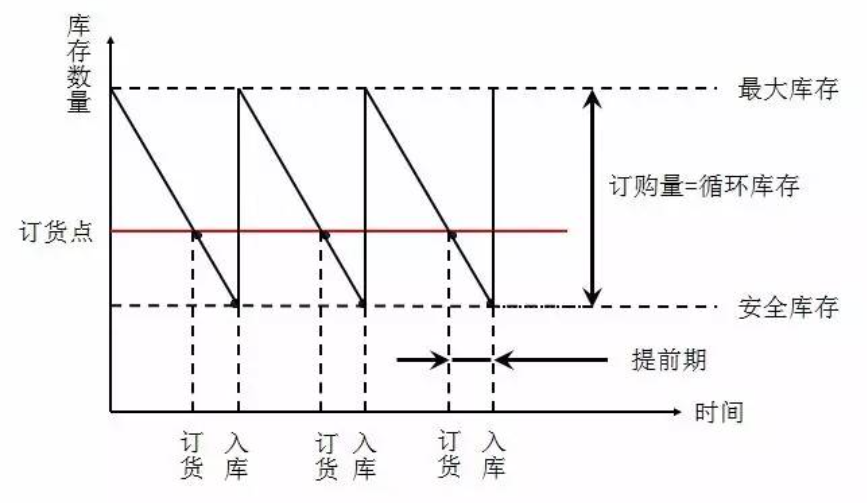
\includegraphics[width=0.6\textwidth]{EOQ.png}
	\caption{经济订购批量模型(EOQ)示意图。}
	\label{fig:eoq}
\end{figure}

经济订购批量模型需要解决两个问题:
\begin{itemize}
 \item 多长时间补充一次货源;
 \item 每次货源补充数量是多少。
\end{itemize}
该模型有不允许缺货,且备货时间短的特点。模型建立的假设条件如下:

\begin{itemize}
 \item 需求是连续的,均匀的,分析期内需求量固定不变;
 \item 当存储降为0时,可立即得到补充(即生产时间或拖后时间很短,可近似地看成0);
 \item 每次订货量不变,记为Q,订购费不变(每次生产量不变,装配费不变);
 \item 不允许缺货,缺货费用无限大;
 \item 单位存储费不变;
\end{itemize}
由于不允许缺货,所以实际上当前该模型只考虑存储费用和订货费用。

在本文的模型中,我们另有如下假设:
\begin{itemize}
 \item 模型中订货提前期为3天;
 \item 库存费用是当前库存的线性函数;
 \item 初始库存为0;
\end{itemize}

定义如下参数:$D$表示B类图书年需求量;$K$表示单位印刷成本,即订货时每次印刷的成本开销;$h$表示每件商品发货费用,在本文中由于假设发货费率不变,则该成本在确定图书类型后作为常数处理;$Q$表示单位订货量;总成本以$C$表示;以$T$代表销售周期长度;日平均需求量为$d$。于是,根据EOQ原理以及默认的模型参数设置,我们有如下模型:
\begin{equation}
\label{eq:eoq}
 C = \frac{KD}{Q} + \frac{hQ}{2} = \frac{KD}{1} + \frac{Q}{2}pc\cdot sr,
\end{equation}
可见当$C$取最小值时,
\begin{equation}
\label{eq:eoq-q}
 Q' = \sqrt{\frac{2KD}{pc\cdot sr}},
\end{equation}

此处由于年需求量$D$与订货量$Q$之间没有严格的数值关系,为了更符合问题二的实际情况,在求总印刷成本时,对印刷次数向上取整。即:
\begin{equation}
\label{eq:kd/q}
 \frac{KD}{Q} >= roundup(\frac{D}{Q})K,
\end{equation}
取再印刷点$R$为$R = roundup(\frac{D}{Q})K$,其中$d=D/T$。

在本题中,基于数据的特征我们有如下分析:

由于印刷成本=上版费+装订费+纸张费+印刷费+印后工艺,除去每次印刷上版费固定,其余值经过验算大致与印刷数量成正比。因此,每件印刷时(装订费+纸张费+印刷费+印后工艺)为常数,略有误差与上版费相比可忽略不计。所以:总印刷成本 =  装订费+纸张费+印刷费+印后工艺。其中:装订费+纸张费+印刷费+印后工艺是与$Q$无关的常数,所以在这里将上版费视为$K$。

\subsubsection{模型检验、方案形成及利润估计}

与问题一类似的,为验证问题二的EOQ模型,我们将所得方案计算总成本$C$和利润$pf$,并与往年的印刷方案总成本及利润对比。

\subsection{问题三}

基于第三章对问题三的分析,该问题的求解主要包括根据销售热度的变化预测接下来的图书销量、结合现有库存判断是否需要重印、重印方案、以所得模型预测结果为基础,形成印刷方案并给出预估利润、评估往年的重印策略是否合理等步骤。在本节,处理这些步骤的方法将一一展开。

\subsubsection{下一年销量预测}


%\renewcommand{\algorithmicrequire}{\textbf{Input:}}
%\renewcommand{\algorithmicensure}{\textbf{Output:}}
%%\removelatexerror
%\begin{algorithm}[t]
%	\caption{种群初始化}
%	\label{alg:init}
%	\begin{algorithmic}[1]
%		\REQUIRE $q$ (待生成初始种群的样本位点测量值),$X$ (操作位点) $NP$ (种群大小), $X_{min},X_{max}$ (变量范围)
%		\ENSURE  $P$ (初始种群)
%		\STATE $//$计算操作位点从样本点出发向上下可调整的次数区间
%		\STATE $//$(以原点为中心,负数则为向下调整,正数为向上调整)
%		\FOR {每个操作位点$x_{i}$}
%			\STATE $u_{i}=\frac{X_{max}^{i}-x_{i}}{\Delta}$
%			\STATE $l_{i}=\frac{x_{i}-X_{max}^{i}}{\Delta}$
%		\ENDFOR
%		\STATE $P=\emptyset$
%		\WHILE {$|P|<NP$}
%		\STATE $//$对每个位点随机选择调整次数,组成初始种群中的一个个体
%		\FOR {$i=1\leftarrow |X|$}
%		\STATE 产生随机数$r,r\in [l_{i},u_{i}]$
%		\STATE $p_{i}=q_{i}+r\times \Delta$
%		\ENDFOR
%		\STATE $ P \leftarrow P \cup p$
%		\ENDWHILE
%		\RETURN $P$
%	\end{algorithmic}
%\end{algorithm}

\newpage

\section{结果分析与检验}

\subsection{问题一}

\subsubsection{下一年销售总量预测}

根据第4.1.1章的模型,我们得到了A类图书往年销售总量的预测数据与下一年销售总量的预测结果,并统计了往年的预测值和实际值的误差率:
\begin{equation}
\label{eq:er}
  er = \frac{sv_p - sv_r}{sv_r},
\end{equation}
其中,$sv_r$和$sv_p$分别代表预测值与实际值。

结果统计如下表~\ref{tab:q1-total},其中包括了A1,A2,A4,A5的预测结果,由于A3直接采用均值作为预测结果,故无需统计。A3的结果为:$sv^3_p=28610$,其他结果如下表展示。

\begin{table}[htbp]
  \centering
  \resizebox{\textwidth}{!}{
    \begin{tabular}{rrrrrrrrrrrrr}
    \toprule
    \multicolumn{1}{l}{布朗模型} & \multicolumn{1}{l}{A1-时间} & \multicolumn{1}{l}{实测数据} & \multicolumn{1}{l}{拟合数据} & \multicolumn{1}{c}{浮动} & \multicolumn{1}{l}{$er$} &       & \multicolumn{1}{l}{ARIMA(0,0,0)} & \multicolumn{1}{l}{A2-时间} & \multicolumn{1}{l}{实测数据} & \multicolumn{1}{l}{拟合数据} & \multicolumn{1}{c}{浮动} & \multicolumn{1}{l}{$er$} \\
    \midrule   
          & 2013  & 133890 & 135518 & 1628  & 0.012159 &       &       & 2015  & 131259 & 144099 & 12840 & 0.097822 \\
          & 2014  & 135870 & 137370 & 1500  & 0.01104 &       &       & 2016  & 142036 & 144099 & 2063  & 0.014524 \\
          & 2015  & 147746 & 138309 & -9437 & -0.06387 &       &       & 2017  & 147520 & 144099 & -3421 & -0.02319 \\
          & 2016  & 153854 & 156399 & 2545  & 0.016542 &       &       & 2018  & 148981 & 144099 & -4882 & -0.03277 \\
          & 2017  & 159517 & 161088 & 1571  & 0.009848 &       &       & 2019  & 141600 & 144099 & 2499  & 0.017648 \\
          & 2018  & 155449 & 165637 & 10188 & 0.065539 &       &       & 2020  & 150500 & 144099 & -6401 & -0.04253 \\
          & 2019  & 154577 & 154771 & 194   & 0.001255 &       &       & 2021  & 146800 & 144099 & -2701 & -0.0184 \\
          & 2020  & 152300 & 153481 & 1181  & 0.007754 &       &       & 2022  &       & 144099 &       &  \\
          & 2021  &       & 150416 &       &       &       &       &       &       &       &       &  \\
\bottomrule
          \toprule  
    \multicolumn{1}{l}{霍尔特} & \multicolumn{1}{l}{A4-时间} & \multicolumn{1}{l}{实测数据} & \multicolumn{1}{l}{拟合数据} & \multicolumn{1}{c}{浮动} & \multicolumn{1}{l}{$er$} &       & \multicolumn{1}{l}{霍尔特} & \multicolumn{1}{l}{A5-时间} & \multicolumn{1}{l}{实测数据} & \multicolumn{1}{l}{拟合数据} & \multicolumn{1}{c}{浮动} & \multicolumn{1}{l}{$er$} \\
    \midrule   
          & 2013  & 101900 & 100665 & -1235 & -0.01212 &       &       & 2013  & 101900 & 100665 & -1235 & -0.01212 \\
          & 2014  & 109900 & 109416 & -484  & -0.0044 &       &       & 2014  & 109900 & 109416 & -484  & -0.0044 \\
          & 2015  & 116100 & 118019 & 1919  & 0.016529 &       &       & 2015  & 116100 & 118019 & 1919  & 0.016529 \\
          & 2016  & 131800 & 126146 & -5654 & -0.0429 &       &       & 2016  & 131800 & 126146 & -5654 & -0.0429 \\
          & 2017  & 134849 & 135772 & 923   & 0.006845 &       &       & 2017  & 134849 & 135772 & 923   & 0.006845 \\
          & 2018  & 141700 & 144096 & 2396  & 0.016909 &       &       & 2018  & 141700 & 144096 & 2396  & 0.016909 \\
          & 2019  & 148940 & 152128 & 3188  & 0.021405 &       &       & 2019  & 148940 & 152128 & 3188  & 0.021405 \\
          & 2020  & 164689 & 160004 & -4685 & -0.02845 &       &       & 2020  & 164689 & 160004 & -4685 & -0.02845 \\
          &    2021   &       & 169438 &       &       &       &       & 2021  &       & 169438 &       &  \\
          \bottomrule
    \end{tabular}%
    }
\caption{A类图书年销售总量预测与实际值,及下一年预测值。}
\label{tab:q1-total}
\end{table}

A1的预测结果位于表格的左上方,从结果中我们可以看出,所有年份的误差率$er$均在10\%以内,最大为6\%,其余都在2\%以下。为更直观地观察和分析,我们将实测数据和拟合数据绘制成折线图,结果如下:
\begin{figure}[H]
	\centering		
	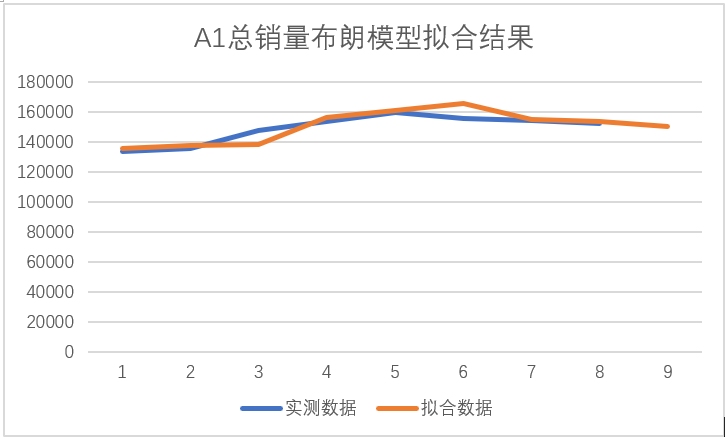
\includegraphics[width=0.6\textwidth]{A1-Q1.PNG}
	\caption{A1总销量布朗模型拟合结果。}
	\label{fig:a1-q1}
\end{figure}
从图中可以直观地看到,拟合结果十分逼近。

A2的预测结果位于表格的右上方。从图中数据可以看出,最终ARIMA拟合结果采用了往年历史数据的算数平均数。这是因为,A2总销量的年变化没有稳定趋势,但总销量较稳定。

A4的预测结果位于表格的左下方,从结果中我们可以看出,所有年份的误差率$er$均在3\%以内,最大为2.8\%。为更直观地观察和分析,我们将实测数据和拟合数据绘制成折线图,结果如下:
\begin{figure}[H]
	\centering		
	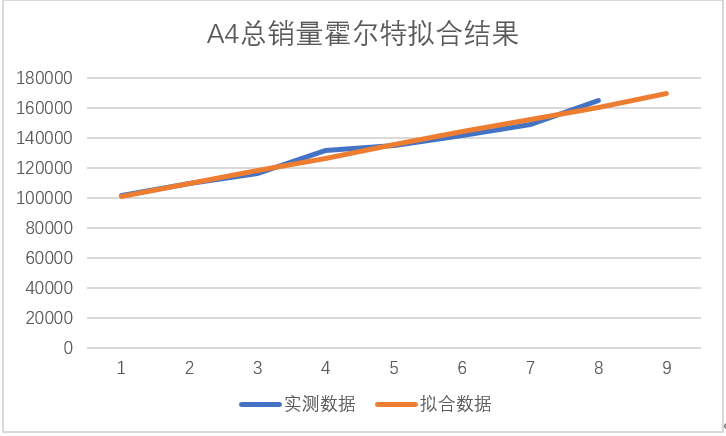
\includegraphics[width=0.6\textwidth]{A4-Q1.PNG}
	\caption{A4总销量霍尔特模型拟合结果。}
	\label{fig:a4-q1}
\end{figure}
从图中可以直观地看到,拟合结果十分逼近。

A5的预测结果位于表格的右下方,从结果中我们可以看出,所有年份的误差率$er$均在5\%以内,最大为4.3\%,其余都在3\%以下。为更直观地观察和分析,我们将实测数据和拟合数据绘制成折线图,结果如下:
\begin{figure}[H]
	\centering		
	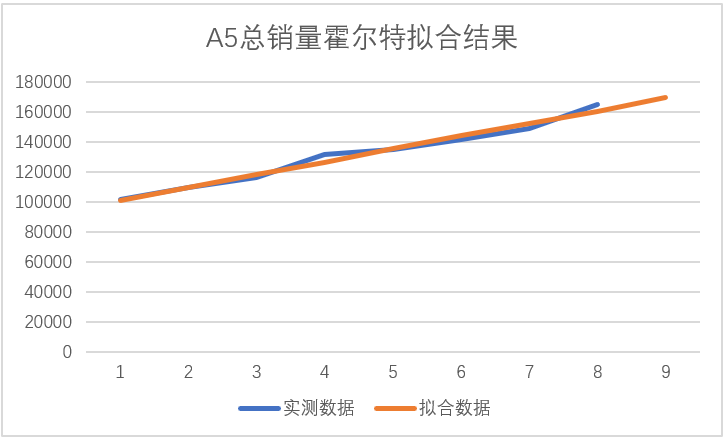
\includegraphics[width=0.6\textwidth]{A5-Q1.PNG}
	\caption{A5总销量霍尔特模型拟合结果。}
	\label{fig:a5-q1}
\end{figure}
从图中可以直观地看到,拟合结果十分逼近。

从表中可以明显看出,对于A1,A2,A4,A5的预测结果,根据往年数据验证,其误差率均在10\%以内,且绝大部分误差率在3\%以内。因此,该模型对下一年总量的预测精度较高。根据该模型,我们给出了所有图书下一年预测值,记录在表~\ref{tab:q1-total}中每一年的最后一列(此外A3的总量为28610)。

\subsubsection{模型性能检验}

之后,为了验证所得模型的精度,根据上述所得预测值,我们在往年数据中挑选了订单总数较多的年份。这些年份的订单根据4.1.2的模型重新规划印次和印数,并计算利润与往年方案对比。结果如下:

\begin{table}[htbp]
  \centering
  \resizebox{0.8\columnwidth}{!}
  {
    \begin{tabular}{crrrrrrrccc}
    \toprule
    \multirow{2}[0]{*}{原A1方案} & \multicolumn{1}{p{4.04em}}{2019秋第1次印数2019.6.18} & \multicolumn{1}{p{4.04em}}{2019秋第2次印数2019.7.5} & \multicolumn{1}{p{4.04em}}{2019秋第3次印数2019.7.10} & \multicolumn{1}{p{4.04em}}{2019秋第4次印数2019.8.12} & \multicolumn{1}{p{4.04em}}{2019秋第5次印数2019.8.26} & \multicolumn{1}{p{4.04em}}{2019秋第6次印数2019.9.2} & \multicolumn{1}{c}{2019秋总印数} & \multicolumn{1}{l}{利润} & \multicolumn{1}{l}{成本} & \multicolumn{1}{l}{\textbf{成本利润率}} \\
          & \multicolumn{1}{c}{100000} & \multicolumn{1}{c}{30000} & \multicolumn{1}{c}{20000} & \multicolumn{1}{c}{2000} & \multicolumn{1}{c}{2000} & \multicolumn{1}{c}{1500} & \multicolumn{1}{c}{155500} & \multirow{2}[0]{*}{463187.8} & \multirow{2}[0]{*}{547189.3} & \multirow{2}[0]{*}{\textbf{0.846485}} \\
    印刷成本  & 306684 & 94266.14 & 63920.76 & 9652.29 & 9652.29 & 9652.29 & 493827.77 &       &       &  \\
    \multirow{2}[0]{*}{改进方案} & \multicolumn{1}{l}{2019.7.18} & \multicolumn{1}{l}{2019.9.9} &       &       &       &       & \multicolumn{1}{c}{总印数} & \multirow{3}[0]{*}{480981} & \multirow{3}[0]{*}{529396.1} & \multirow{3}[0]{*}{\textbf{0.908546}} \\
          & 151668 & 3034  &       &       &       &       & \multicolumn{1}{c}{154702} &       &       &  \\
    印刷成本  & 463472.3 & 12836.12 &       &       &       &       & 476308.44 &       &       &  \\
\midrule
    \multirow{2}[0]{*}{原A2方案} & \multicolumn{1}{p{4.04em}}{2016春第1次印数2015.12.11} & \multicolumn{1}{p{4.04em}}{2016春第2次印数2015.12.28} & \multicolumn{1}{p{4.04em}}{2016春第3次印数   2016.2.1} & \multicolumn{1}{p{4.04em}}{2016春第4次印数   2016.3.4} &       &       & \multicolumn{1}{c}{2016春总印数} & \multicolumn{1}{l}{利润} & \multicolumn{1}{l}{成本} & \multicolumn{1}{l}{\textbf{成本利润率}} \\
          & \multicolumn{1}{c}{126000} & \multicolumn{1}{c}{15000} & \multicolumn{1}{c}{1000} & \multicolumn{1}{c}{138} &       &       & \multicolumn{1}{c}{142138} & \multirow{2}[0]{*}{370251.6} & \multirow{2}[0]{*}{491679.6} & \multirow{2}[0]{*}{\textbf{0.753034}} \\
    印刷成本  & 385581.8 & 48748.07 & 7559.111 & 4506.758 &       &       & 446395.729 &       &       &  \\
    \multirow{2}[0]{*}{改进方案} & \multicolumn{1}{l}{2015.12.7} & \multicolumn{1}{l}{2016.1.5} & \multicolumn{1}{l}{2016.2.20} &       &       &       & \multicolumn{1}{c}{总印数} & \multirow{3}[0]{*}{368537.6} & \multirow{3}[0]{*}{493393.6} & \multirow{2}[0]{*}{\textbf{0.746944}} \\
          & \multicolumn{1}{c}{119127} & 23200 & 1500  &       &       &       & \multicolumn{1}{c}{143827} &       &       &  \\
    印刷成本  & 364725.4 & 73631.28 & 9214.95 &       &       &       & 447571.65 &       &       &  \\
\midrule
    \multirow{2}[0]{*}{原A3方案} & \multicolumn{1}{p{4.04em}}{2014秋第1次印数2014.8.8} & \multicolumn{1}{p{4.04em}}{2014秋第2次印数2014.8.29} & \multicolumn{1}{p{4.04em}}{2014秋第3次印数2014.8.18} & \multicolumn{1}{p{4.04em}}{2014秋第4次印数2014.8.22} & \multicolumn{1}{p{4.04em}}{2014秋第5次印数2014.8.27} &       & \multicolumn{1}{c}{2014秋总印数} & \multicolumn{1}{l}{利润} & \multicolumn{1}{l}{成本} & \multicolumn{1}{l}{\textbf{利润率}} \\
          & \multicolumn{1}{c}{12000} & \multicolumn{1}{c}{2000} & \multicolumn{1}{c}{2000} & \multicolumn{1}{c}{8000} & \multicolumn{1}{c}{5000} &       & \multicolumn{1}{c}{29000} & \multirow{2}[0]{*}{-11967} & \multirow{2}[0]{*}{115189.2} & \multirow{2}[0]{*}{\textbf{-0.10389}} \\
    印刷成本  & 39644.46 & 9652.29 & 9652.29 & 28127.15 & 18889.72 &       & 105965.91 &       &       &  \\
    \multirow{2}[0]{*}{改进方案} & \multicolumn{1}{l}{2014.8.20} & \multicolumn{1}{l}{2014.9.21} &       &       &       &       & \multicolumn{1}{c}{总印数} & \multirow{3}[0]{*}{38998.89} & \multirow{3}[0]{*}{64223.38} & \multirow{2}[0]{*}{\textbf{0.607238}} \\
          & \multicolumn{1}{c}{14579} & 2538  &       &       &       &       & \multicolumn{1}{c}{17117} &       &       &  \\
    印刷成本  & 47470.53 & 11308.87 &       &       &       &       & 58779.4 &       &       &  \\
    \midrule
    \multirow{2}[0]{*}{原A4方案} & \multicolumn{1}{p{4.04em}}{2018秋第1次印数2018.6.29} & \multicolumn{1}{p{4.04em}}{2018秋第2次印数2018.7.9} & \multicolumn{1}{p{4.04em}}{2018秋第3次印数2018.7.11} & \multicolumn{1}{p{4.04em}}{2018秋第4次印数2018.7.19} & \multicolumn{1}{p{4.04em}}{2018秋第5次印数2018.9.13} &       & \multicolumn{1}{c}{2018秋总印数} & \multicolumn{1}{l}{利润} & \multicolumn{1}{l}{成本} & \multicolumn{1}{l}{\textbf{利润率}} \\
          & \multicolumn{1}{c}{110000} & \multicolumn{1}{c}{12500} & \multicolumn{1}{c}{13200} & \multicolumn{1}{c}{4300} & \multicolumn{1}{c}{2000} &       & \multicolumn{1}{c}{142000} & \multirow{2}[0]{*}{338987.5} & \multirow{2}[0]{*}{442062.9} & \multirow{2}[0]{*}{\textbf{0.766831}} \\
    印刷成本  & 301719.2 & 36847.86 & 38749.5 & 14993.61 & 8660.8 &       & 400970.93 &       &       &  \\
    \multirow{2}[0]{*}{改进方案} & \multicolumn{1}{l}{2018.7.22} &       &       &       &       &       & \multicolumn{1}{c}{总印数} & \multirow{3}[0]{*}{349178.9} & \multirow{3}[0]{*}{431871.5} & \multirow{2}[0]{*}{\textbf{0.808525}} \\
          & \multicolumn{1}{c}{142708} &       &       &       &       &       & \multicolumn{1}{c}{142708} &       &       &  \\
    印刷成本  & 390574.7 &       &       &       &       &       & 390574.66 &       &       &  \\
     \midrule
    \multirow{2}[0]{*}{原A5方案} & \multicolumn{1}{p{4.04em}}{2020春第1次印数2019.11.26} & \multicolumn{1}{p{4.04em}}{2020春第2次印数2019.11.28} & \multicolumn{1}{p{4.04em}}{2020春第3次印数2019.12.5} & \multicolumn{1}{p{4.04em}}{2020春第4次印数2019.12.10} & \multicolumn{1}{p{4.04em}}{2020春第5次印数2019.12.16} & \multicolumn{1}{p{4.04em}}{2020春第6次印数2020.1.3} & \multicolumn{1}{c}{2020春总印数} & \multicolumn{1}{l}{利润} & \multicolumn{1}{l}{成本} & \multicolumn{1}{l}{\textbf{利润率}} \\
          & \multicolumn{1}{c}{90000} & \multicolumn{1}{c}{20000} & \multicolumn{1}{c}{27000} & \multicolumn{1}{c}{3500} & \multicolumn{1}{c}{6800} & \multicolumn{1}{c}{2000} & \multicolumn{1}{c}{149300} & \multirow{2}[0]{*}{375105.8} & \multirow{2}[0]{*}{468604.3} & \multirow{2}[0]{*}{\textbf{0.800474}} \\
    印刷成本  & 247386.6 & 57222.57 & 76238.98 & 12790.89 & 21877.11 & 8661  & 424177.14 &       &       &  \\
    \multirow{2}[0]{*}{改进方案} & \multicolumn{1}{l}{2019.12.6} & \multicolumn{1}{l}{2020.1.3} & \multicolumn{1}{l}{2020.1.27} &       &       &       & \multicolumn{1}{c}{总印数} & \multirow{3}[0]{*}{382585.3} & \multirow{3}[0]{*}{461124.8} & \multirow{2}[0]{*}{\textbf{0.829678}} \\
          & 137017 & 11116 & 1500  &       &       &       & \multicolumn{1}{c}{149633} &       &       &  \\
    印刷成本  & 375114.3 & 33107.49 & 8376.715 &       &       &       & 416598.525 &       &       &  \\
    \bottomrule
    \end{tabular}%
    }
  \label{tab:verify}
  \caption{安全库存模型结果与原数据,在A1-A5中印次最高的年份方案对比。}
\end{table}

对于A1图书,原方案下,2019年秋印次高达6次,带来的总成本为54万多,利润为46万多;而采用我们的模型得到的方案下,印次控制在2次,且成本大大降低,为529万多,利润同时有所增高,为481万左右。计算所得利润率,较原方案的85\%,改进方案提升为91\%。

对于A2图书,原方案下2016年春印次为4,成本为49万左右,利润为37万;采用我们的模型可以将印次降低为2次,成本有略微的提升,为49万,利润也略微有所降低,为37万。该方案下印次能够降低为2,但利润率降低了不到1\%。

对于A3图书,原方案下,2014年秋印次5次,成本为11万,利润则是-1万多;而我们的改进方案下,印次降低为2次,成本缩减为6万多,利润提高到3万8千多,利润率达到61\%。

对于A4图书,原方案下,2018年秋印次高达5次,成本为44万,利润为33万;我们的方案只需要1次印次,成本为43万,利润为35万左右。相比原方案,利润率提高了3.4\%。

对于A5图书,原方案下,2020年春印次高达6次,成本为46万,利润为37万;我们的方案只需要3次印次,且成本略微降低,而利润增高了近1万。总的来说,利润率提升了接近3\%。

从上表所示的结果我们可以看到,除了A2的成本有少许提高外,其余A1,A2,A3和A5,模型给出的方案都能将印次控制在3以内并降低成本。所以我们可以验证得到,我们提出的安全库存模型能够适用于问题一的情景。

在该模型的基础上,应对接下来的一年,我们只需要按照上述4.1的处理过程,在订单的动态变化下,对下一年的销售通过该模型给出方案即可。通过这一模型,印次可以控制在3次以内,而且能够实现更高的利润。

\subsection{问题二}

\subsubsection{EOQ模型相关系数分析结果}

把相关系数的表格结果写上去,并且对重要参数进行分析

\subsubsection{EOQ模型规划结果模拟}

把EOQ结果示意图的结果写上去,并且根据当时讨论的,对曲线图进行详细分析

\subsubsection{方案形成及利润估计}

根据EOQ模型给出下一年的印刷方案,计算利润

\newpage

\section{总结}

本文旨在求解工业中尚待研究的汽油辛烷值优化问题,

由于时间有限、我们队伍的学术研究水平也有限,论文中可能存在许多排版、内容上的疏漏。在解题过程中,我们也发现了许多问题,其中有很多都没能得到解决。主要包括如下:
\begin{itemize}
	\item 本题中
\end{itemize}


\begin{thebibliography}{9}
 \bibitem{bib:one}薛冬梅.ARIMA模型及其在时间序列分析中的应用[J].吉林化工学院学报,2010,27(03):80-83.
 \bibitem{bib:two}郑月. 不同时间序列分析法在全国公共图书馆机构数预测中的比较[D].广西师范大学,2021.
 \bibitem{bib:three}杨真真,郭贝贝,孙艳彬.基于SPSS的指数平滑模型及实例[J].中国科技信息,2021(13):74-75.
 \bibitem{bib:four}张琼,张爱华.霍尔特指数平滑法在商品销量预测中的应用[J].市场论坛,2012(03):70-71.
 \bibitem{bib:five}王惠文, 孟洁."多元线性回归的预测建模方法." 北京航空航天大学学报 .04(2007):500-504.
 \bibitem{bib:six}周志华.机器学习[M].北京: 清华大学出版社,2016: page 24-26,53-55,127-138.
 \bibitem{bib:seven}ZHOU Zhi hua, HE, YIN, CHEN. (2001). A statistics-based approach for rule extraction from neural networks. Journal of Software.
\end{thebibliography}

\bibliographystyle{gmcm}

\end{document} 